\documentclass[12pt,a4paper]{article}

\usepackage{float}
\restylefloat{figure}
\usepackage{hyperref}
\usepackage{graphicx}
\usepackage{gensymb}
\usepackage[title]{appendix}
\usepackage[dotinlabels]{titletoc}
\usepackage[nottoc,numbib]{tocbibind}
\usepackage{mathtools}
\usepackage[margin=0.5in]{geometry}
\renewcommand{\thefootnote}{\arabic{footnote}}

\newcommand*\wrapletters[1]{\wr@pletters#1\@nil}
\def\wr@pletters#1#2\@nil{#1\allowbreak\if&#2&\else\wr@pletters#2\@nil\fi}

\usepackage{enumitem}
\setenumerate{itemsep=0pt}

% Add support for multi-page tables.
\usepackage{longtable}

\pagenumbering{arabic}

\title{EE4DSA Coursework 3}
\author{Chris Cummins}

\begin{document}
\maketitle

\section{Disassembling the program ROM}

The file \texttt{extra/ram.asm} contains a heavily annotated
disassembled version of the safe unlocking program in a style inspired
by the AVR Assembler Syntax. The program tests for the safe code 2013.

The assembly code was generated automatically using a disassembler
developed for this purpose, available at
\url{http://chriscummins.cc/disassembler}. Based off of the
implementation of the second coursework disassembler, the
functionality has been extended to support ALU and register file
instructions.

\begin{figure}[H]
  \centering
  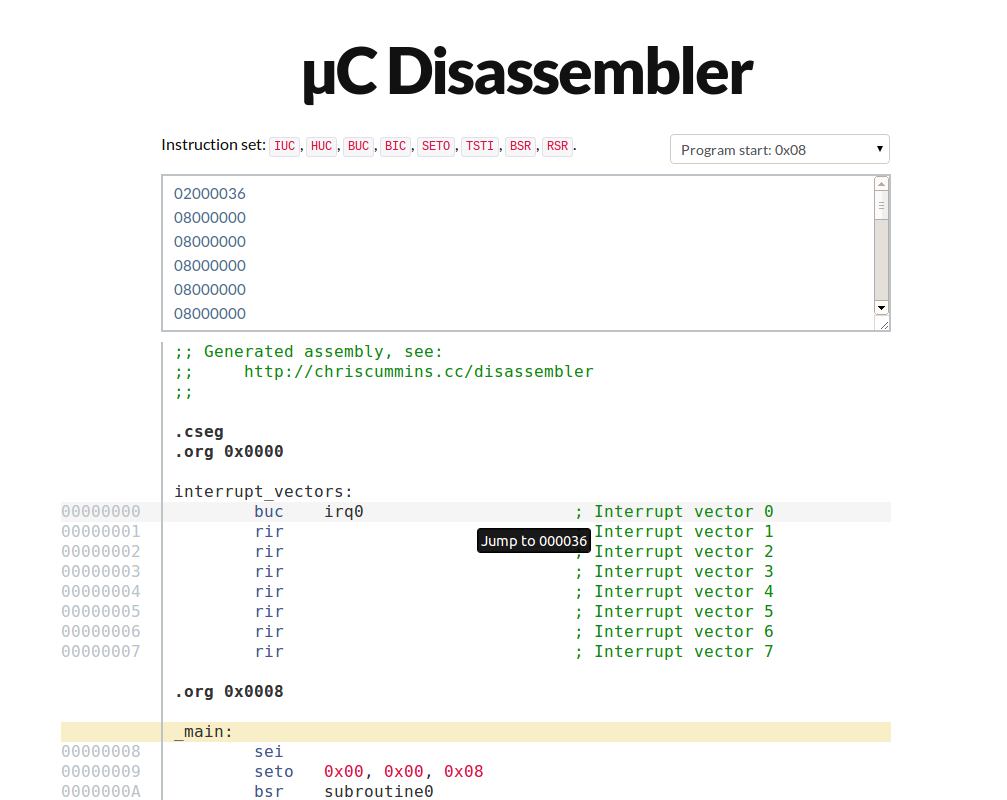
\includegraphics[width=6.7in]{assets/disassembler.png}
\end{figure}

A standalone version is available in \texttt{extra/disassembler}, and
contains the following files:

\begin{itemize}
\item \texttt{ee4dsa-util.js} - Utility functions for working with
  JavaScript types and performing numerical base conversions.
\item \texttt{ee4dsa-asm.js} - Contains objects used to render parts
  of assembly programs, such as instructions, comments, directives
  etc.
\item \texttt{ee4dsa-disassembler.js} - Provides functions to decode
  RAM dumps into sets of assembly components, and to produce
  representations of programs. Implements the actual instruction set
  and machine code parser.
\item \texttt{index.html} - Markup and JavaScript to implement the
  disassembler.
\end{itemize}

\section{Implementing the EU \& ALU}

The file \texttt{execution\_unit.vhd} contains my implementation of
the execution unit. The first step upon importing the coursework 2
implementation was to refactor out the \texttt{next\_pc\_src}
multiplexer, allowing the instruction set process to set the next
program counter directly. While slightly obfuscating the code (the
\texttt{next\_pc} signal is now assigned in multiple places), this did
provide a 10 MHz increase in the maximum operating frequency,
providing the required performance needed to implement the register
file and ALU instructions. Since the ALU has no internal states, the
ALU required only a single level of immediate logic.

\section{Synthesising the design}

The directory \texttt{reports/} contains a copy of the synthesis
reports. The design synthesis without pertinent warnings:

\begin{verbatim}
$ make synthesis
Synthesis running...
WARNING:HDLCompiler:634 - "/home/chris/src/vhdl-exercises/ee4dsa/cw3/top_level.vhd" \
  Line 112: Net <eu_intr[7]> does not have a driver.
WARNING:Xst:2935 - Signal 'eu_intr<7:2>', unconnected in block 'top_level', is tied \
  to its initial value (000000).
\end{verbatim}

Analysing the log \texttt{reports/xst.log} shows that the maximum
achievable frequency of the design is 105.029 MHz. The bottlenecks in
this performance are the large fanout involved in the
\texttt{next\_pc\_srrc} multiplexer, and the number of different
assignments to the \texttt{next\_[bc]\_reg\_addr} registers.

The fact that 66.2\% of the longest data path is in the route and not
logic shows that it is the delay in transmission speed which is
preventing higher performance, and this could be increased by reducing
the number of different places in which registers are assigned,
leading to fewer input multiplexers and shorter paths between
components.

\newpage
\begin{verbatim}
=========================================================================
Timing constraint: Default period analysis for Clock 'clk'
  Clock period: 9.521ns (frequency: 105.029MHz)
  Total number of paths / destination ports: 458963 / 1903
-------------------------------------------------------------------------
Delay:               9.521ns (Levels of Logic = 5)
  Source:            ram_unit/Mram_data7 (RAM)
  Destination:       ram_unit/Mram_data1 (RAM)
  Source Clock:      clk rising
  Destination Clock: clk rising

  Data Path: ram_unit/Mram_data7 to ram_unit/Mram_data1
                                Gate     Net
    Cell:in->out      fanout   Delay   Delay  Logical Name (Net Name)
    ----------------------------------------  ------------
     RAMB16BWER:CLKB->DOB0  137   1.850   2.222  ram_unit/Mram_data7 (eu_rom_data<24>)
     LUT6:I2->O            4   0.203   0.684  execution_unit/_n4252<29>1              \
       (execution_unit/_n4252)
     LUT3:I2->O           11   0.205   0.883  execution_unit/Mmux_next_pc_src<0>341   \
       (execution_unit/Mmux_next_pc_src<0>34)
     LUT6:I5->O           11   0.205   0.883  execution_unit/Mmux_next_pc_src<0>343_2 \
       (execution_unit/Mmux_next_pc_src<0>343_1)
     LUT3:I2->O            1   0.205   0.827  execution_unit/Mmux_next_pc33_SW0 (N290)
     LUT6:I2->O            8   0.203   0.802  execution_unit/Mmux_next_pc33           \
       (eu_rom_addr<3>)
     RAMB16BWER:ADDRB5         0.350          ram_unit/Mram_data1
    ----------------------------------------
    Total                      9.521ns (3.221ns logic, 6.300ns route)
                                       (33.8% logic, 66.2% route)
\end{verbatim}

\end{document}
